\documentclass{article}
\usepackage{amssymb, amsmath, amsthm}
\usepackage[margin=1in]{geometry}
\usepackage{verbatim}
\usepackage{graphicx}
\usepackage{hyperref} % \url \href
\usepackage{docmute}

\newtheorem{definition}{Definition}
\newtheorem{theorem}{Theorem}
\newcommand{\heff}{\mathbb{H}^{\text{eff}}}
\newcommand{\pfrac}[2]{\frac{\partial #1}{\partial #2}}

\newcommand{\MO}{\textbf{MO}}
\newcommand{\AO}{\textbf{AO}}

\newcommand{\huptb}{\text{H}_0}
\newcommand{\order}[2]{#1^{(#2)}}
\newcommand{\statebra}[1]{\langle #1 |}
\newcommand{\stateket}[1]{| #1 \rangle}

\begin{document}

\section{Through-bond Interaction}
In this section, we provide example of how the presense of some bonds 
affect other bonds in molecular. As we can see, such bond-bond interaction 
can be understood following the consideration of molecular orbital 
perturbation treatment. 

\subsection{Bond-bond Interaction}
Let's consider the molecular orbital of C$_3$H$_6$ and its variant to illustrate the 
how the presense of orbitals change the interaction between other bonds and eventually the 
geometry of the molecular structure. First, let's construct the molecular orbital diagram 
of the C$_3$H$_6$ molecular itself. Instead of starting from the entire molecular, we first 
consider the MO diagram of the CH$_2$ fragments.  

\subsection{Through-bond Interaction}
Let's define two different kind of orbital interaction:
\begin{enumerate}
    \item Through-space interaction, where $H_{\mu\nu}$ is relatively large and the level splitting is due to these off-diagonal elements
    \item Through-bond interaction, where $H_{\mu\nu}$ is very small but orbital splitting suggest non-ignorable interactions. 
\end{enumerate}
The following example illustrate the through-bond interaction, which is esentially a restatement of the delocalization 
nature of the molecular orbitals. Let's consider the following molecular formed by bringing two NH$_3$ molecular together. 
For each NH$_3$ molecular, we have lone pair electrons pointing opposite to the H atoms. 

The direct, through space interaction between the two lone pair electrons on each side of the molecular is very small, so 
naturally, we expect to see two energy levels, one slightly bonding and one slightly antibonding, very close in energy, as 
shown in figure \ref{F:N2H6_lone_pairs}. \emph{However, the actual splitting of the orbitals are larger than given by 
through-space interaction only} because we ignored the orbitals that are formed between the hydrogens. 

\begin{figure}
    \centering
    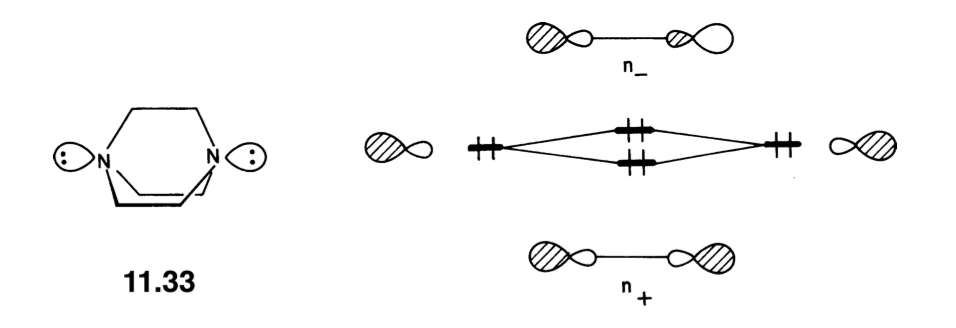
\includegraphics[width=3in]{figures/F_non_interacting_lone_pair.png}
    \caption{N$_2$H$_6$ molecular on the left and the through-space bonding interaction of the lone pairs}
    \label{F:N2H6_lone_pairs}
\end{figure}

To include the effect of other orbitals, we should apply the perturbation treatment on the slightly bonding and antibonding 
molecular orbitals formed in the isolated case by introducing interactions between them and other molecular orbitals. This 
is shown in figure \ref{F:through-bond} for a simplified situation, now it is straight-forward to see that, while the 
perturbation corrected $n_-$ and $n_+$ orbitals are similar to their unperturbed parts, other orbitals start to 
mix in. It can be seen that now the ``antibonding'' $n_-$ orbitals lie at a lower energy because the mixing with 
another higher energy antibonding orbitals. The situation is reversed for the bonding $n_+$ orbitals. As a result, 
the relatively position of the two orbitals are changed due to the presense of other molecular orbitals. Due to the delocalized 
nature of the formed molecular orbitals, it appears \emph{as if} these orbitals have a larger interaction.

\begin{figure}
    \centering
    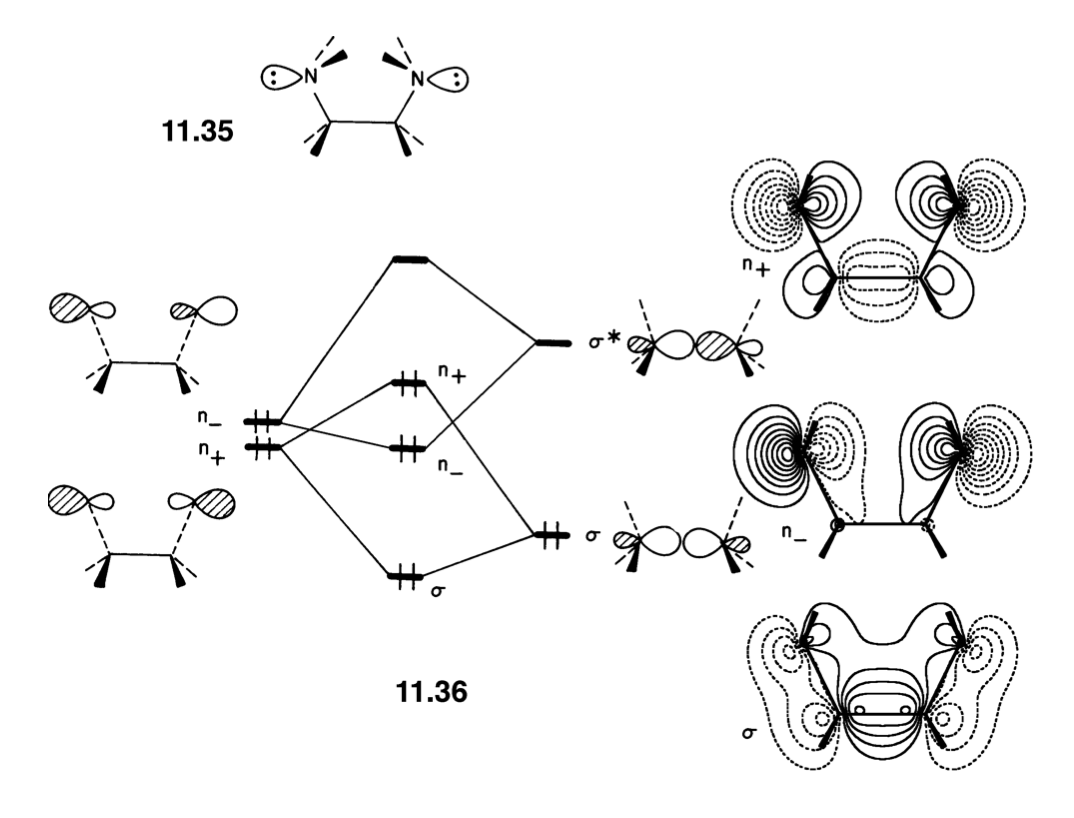
\includegraphics[width=3in]{figures/F_through_bond.png}
    \caption{The effect of other molecular orbitals on the long range interactions}
    \label{F:through-bond}
\end{figure}

\end{document}
